\documentclass[conference]{IEEEtran}
\IEEEoverridecommandlockouts
\usepackage{cite}
\usepackage{amsmath,amssymb,amsfonts}
\usepackage{algorithmic}
\usepackage{graphicx}
\usepackage{textcomp}
\usepackage{xcolor}
\usepackage{array}
\usepackage{booktabs}
\usepackage{multirow}
\usepackage{url}
\usepackage[utf8]{inputenc}
\usepackage[english]{babel}
\usepackage{tikz}
\usetikzlibrary{shapes.geometric, arrows.meta, positioning}

% Define TikZ styles after babel to avoid conflicts
\tikzset{
    startstop/.style = {rectangle, rounded corners, minimum width=2.5cm, minimum height=0.8cm, text centered, draw=black, fill=blue!15},
    process/.style = {rectangle, minimum width=2.5cm, minimum height=0.8cm, text centered, draw=black, fill=orange!20},
    decision/.style = {diamond, minimum width=2cm, minimum height=1cm, text centered, draw=black, fill=yellow!15},
    arrow/.style = {thick, ->, >=stealth}
}

\def\BibTeX{{\rm B\kern-.05em{\sc i\kern-.025em b}\kern-.08em
    T\kern-.1667em\lower.7ex\hbox{E}\kern-.125emX}}

\begin{document}

\title{Comparative Analysis of Particle Swarm Optimization (PSO) and Optuna for Academic Performance Prediction in Peruvian Basic Education}

\author{\IEEEauthorblockN{Beatriz Umiña Machaca}
\IEEEauthorblockA{\textit{Faculty of Statistical and Computer Engineering} \\
\textit{Universidad Nacional del Altiplano Puno}\\
Puno, Peru \\
beatrizuminamachaca@gmail.com}
}

\maketitle

\begin{abstract}
This article presents a comparative methodology for predicting student academic performance through Swarm Intelligence techniques, specifically the Particle Swarm Optimization (PSO) algorithm, applied to hyperparameter tuning of machine learning models. The study is based on real data from the 2022 Sample Evaluation of Peru's Ministry of Education, comprising 7839 records of sixth-grade students, including scores on standardized reading and mathematics tests, as well as socioeconomic, demographic, and contextual variables from the country's 25 regions. The proposed PSO approach is compared with Bayesian optimization using the Optuna framework through 5-fold cross-validation for both evaluated subjects. Results demonstrate statistically equivalent performance between both methods in both curricular areas. In reading, the PSO-optimized model achieved a Mean Squared Error (MSE) of 4872 ± 106 and a coefficient of determination (R²) of 0.203 ± 0.016, while Optuna achieved an MSE of 4872 ± 112 and an R² of 0.203 ± 0.016. In mathematics, PSO obtained an MSE of 6650 ± 261 and R² of 0.154 ± 0.021, compared to Optuna which achieved MSE of 6651 ± 262 and R² of 0.154 ± 0.021. Student's t-tests confirmed the absence of statistically significant differences (p > 0.05) in both subjects. Computational efficiency analysis revealed differentiated patterns by subject: in reading, PSO demonstrated greater efficiency using 88 trees versus 177 for Optuna, while in mathematics, Optuna was more efficient with 152 trees compared to 180 for PSO. Territorial analysis evidenced critical educational inequalities, with coastal departments like Callao (575.29 points), Tacna (565.47), and Lima (561.29) significantly surpassing Amazonian regions like Loreto (453.50), San Martín (490.45), and Huánuco (497.41), generating a territorial gap of 121.79 points equivalent to approximately 1.7 years of schooling. The study concludes that both PSO and Bayesian optimization represent methodologically equivalent alternatives for hyperparameter tuning in educational contexts, with method selection depending on available computational resources and specific subject matter. PSO offers greater implementation simplicity and efficiency in reading, while Optuna provides greater methodological sophistication and efficiency in mathematics. This equivalence is particularly relevant for educational institutions with limited computational resources, enabling selection based on specific operational criteria and contributing to the development of early warning systems for identifying students at academic risk.
\end{abstract}

\begin{IEEEkeywords}
Educational data mining, academic performance prediction, particle swarm optimization, metaheuristics, hyperparameter tuning, Peruvian educational evaluation, machine learning models, cross-validation, territorial educational analysis
\end{IEEEkeywords}

\section{Introduction}

Educational Data Mining has emerged as a fundamental discipline for analyzing large volumes of information from educational systems, using advanced statistical techniques and machine learning algorithms to detect critical variables that influence student academic performance \cite{romero2020educational}. Predictive models in education provide empirical evidence for developing effective public policies and enable early interventions through timely identification of students at academic risk \cite{baker2014educational}.The Peruvian educational system presents significant socioeconomic gaps and regional heterogeneities that limit academic performance, evidenced in territorial disparities that exceed 120 points between coastal and Amazonian departments. Data from national evaluations such as the 2022 Sample Evaluation constitute a strategic source for applying educational data mining techniques in the context of these structural inequalities. The development of robust predictive models faces critical methodological challenges, including hyperparameter optimization and rigorous selection of predictive variables that allow identifying territorial and socioeconomic patterns determining student performance \cite{dutt2017systematic}.In the realm of hyperparameter optimization, two main approaches with promising applications in educational contexts have emerged. Bio-inspired algorithms, especially Swarm Intelligence through Particle Swarm Optimization (PSO), perform efficient searches in complex multidimensional spaces with moderate computational requirements \cite{kennedy1995particle}. Simultaneously, Bayesian optimization methods, implemented in frameworks like Optuna, use probabilistic models to guide future searches more efficiently through sophisticated algorithms like Tree-structured Parzen Estimator (TPE) \cite{bergstra2013making}.Particle Swarm Optimization has consolidated as an effective tool for model adjustment due to its computational simplicity, minimal dependence on derivative calculation, and ability to escape local optima \cite{kennedy1995particle}. This characteristic is particularly relevant for educational institutions with limited computational resources. Optuna has emerged as a leading framework through its TPE algorithm implementation, distinguished by its rapid convergence, automatic pruning capability, and adaptive optimization that can be more efficient in specific contexts \cite{akiba2019optuna}.This study systematically compares PSO against Optuna using real data from the 2022 Sample Evaluation of Peruvian sixth-grade students, evaluating the effectiveness of both methods in predicting academic performance in reading and mathematics. The research contributes to the field of metaheuristic optimization and data-driven educational analysis, providing empirical evidence on methodological equivalence between bio-inspired and Bayesian approaches. The incorporated territorial analysis allows identifying critical geographical patterns requiring differentiated interventions, offering practical recommendations for researchers and educational managers in limited-resource contexts.In this context, the research question arises: What is the comparative effectiveness of Particle Swarm Optimization (PSO) versus Bayesian optimization (Optuna) in terms of predictive accuracy and computational efficiency for predicting academic performance in reading and mathematics with Peruvian educational data, and what territorial implications emerge from the predictive analysis?

\section{Literature Review}

Particle Swarm Optimization (PSO), proposed by Kennedy and Eberhart \cite{kennedy1995particle}, has demonstrated effectiveness in continuous optimization tasks and model adjustment in complex domains \cite{liu2020improved}. In the educational domain, PSO has been used to predict academic performance on virtual platforms \cite{zhang2021learning} and optimize classification models to detect at-risk students \cite{sultana2021pso}. In Latin America, González et al. \cite{gonzalez2023edmcolombia} applied PSO to Colombian school data obtaining notable improvements in predictive accuracy.Simultaneously, Bayesian optimization has revolutionized hyperparameter tuning through frameworks like Optuna, which implements the Tree-structured Parzen Estimator (TPE) algorithm \cite{akiba2019optuna}. Optuna is distinguished by its rapid convergence, automatic pruning of unpromising configurations, and integration with machine learning libraries \cite{feurer2019hyperparameter}. Its application in educational environments has shown promising results in student performance prediction \cite{yang2022optunaed}.Educational Data Mining (EDM) has emerged as a key discipline for discovering patterns that enable predicting outcomes and personalizing learning experiences \cite{romero2020educational, baker2014educational}. In Latin America, EDM implementation faces technical and institutional limitations \cite{pena2014educational}, requiring contextualization according to specific social realities. Studies on territorial educational inequalities have documented persistent performance gaps between urban and rural regions \cite{williamson2020datafication}.In the Peruvian context, data from the 2022 Sample Evaluation \cite{minedu2022em} offer significant potential for advanced predictive models. The comparison between PSO and Optuna is particularly relevant as they represent complementary optimization philosophies: implementation simplicity versus methodological sophistication, especially important in educational contexts with limited resources.

\section{Methodology}

\subsection{Dataset and Variables}
This study uses microdata from the 2022 Sample Evaluation of Peru's Ministry of Education, specifically the dataset corresponding to sixth grade of primary education. The sample comprises 7839 students distributed across the country's 25 regions, guaranteeing representative geographical coverage of urban and rural areas \cite{minedu2022em}. The target variables correspond to standardized reading and mathematics scores, measured on a continuous scale from 0 to 1000 points. The dataset includes six categorical predictor variables that allow analyzing both individual and territorial factors influencing academic performance: gender (Male, Female), mother tongue (Spanish, Quechua, Aymara, others), educational management (State, Non-state), geographical area (Rural, Urban), socioeconomic level (Very low, Low, Medium, High), and department of residence (25 categories).

\begin{table}[htbp]
\caption{Dataset variables}
\resizebox{\columnwidth}{!}{
\begin{tabular}{lll}
\hline
\textbf{Variable} & \textbf{Type} & \textbf{Description} \\
\hline
\texttt{reading\_score} & Numerical & Reading score (0-1000) \\
\texttt{math\_score} & Numerical & Mathematics score (0-1000) \\
\texttt{gender} & Categorical & Student gender \\
\texttt{mother\_tongue} & Categorical & Primary household language \\
\texttt{management} & Categorical & Institution type (State/Non-state) \\
\texttt{area} & Categorical & Geographical location (Rural/Urban) \\
\texttt{socioeconomic\_level} & Categorical & Socioeconomic stratum (4 levels) \\
\texttt{department} & Categorical & Department of residence (25 categories) \\
\hline
\end{tabular}
}
\label{tab:variables}
\end{table}

\subsection{Optimization Models and Validation}
Random Forest was employed as the base algorithm due to its robustness against mixed categorical variables, resistance to overfitting, and capacity to handle non-linear interactions between predictor variables. The optimized hyperparameters were the number of trees (\texttt{n\_estimators}) with range [10, 200] and maximum depth (\texttt{max\_depth}) with range [3, 20].

Two methodological approaches were implemented for optimization. PSO was configured with 20 particles and 50 maximum iterations, using the \texttt{pyswarm} library with standard inertia and acceleration parameters. Optuna was implemented through the Tree-structured Parzen Estimator algorithm with 50 evaluations, applying automatic pruning for unpromising configurations. The PSO algorithm implements fundamental principles of swarm intelligence where each particle represents a candidate solution in the hyperparameter space. Figure~\ref{fig:pso_algorithm} illustrates the particle swarm optimization process developed for this study.

\begin{figure}[htbp]
\centerline{
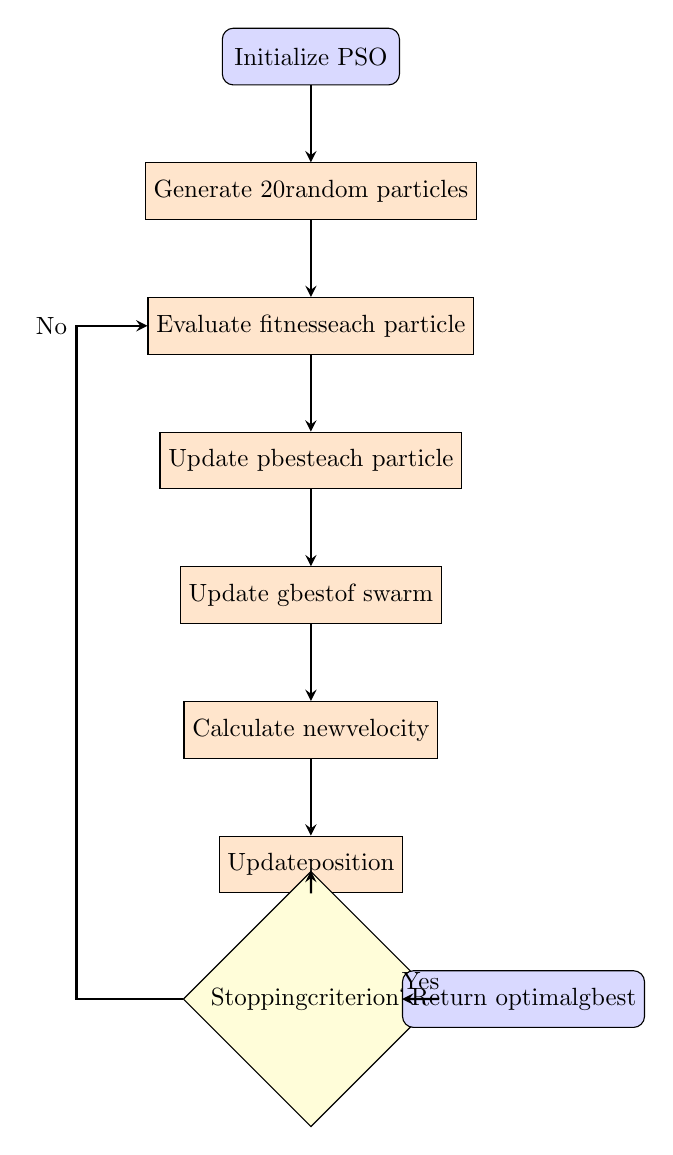
\begin{tikzpicture}[node distance=1.9cm, scale=0.9, transform shape]

\node (inicio) [startstop] {Initialize PSO};
\node (generar) [process, below of=inicio] {Generate 20\\random particles};
\node (evaluar) [process, below of=generar] {Evaluate fitness\\each particle};
\node (actualizarp) [process, below of=evaluar] {Update pbest\\each particle};
\node (actualizarg) [process, below of=actualizarp] {Update gbest\\of swarm};
\node (velocidad) [process, below of=actualizarg] {Calculate new\\velocity};
\node (posicion) [process, below of=velocidad] {Update\\position};
\node (criterio) [decision, below of=posicion] {Stopping\\criterion?};
\node (resultado) [startstop, right of=criterio, node distance=3cm] {Return optimal\\gbest};

\draw [arrow] (inicio) -- (generar);
\draw [arrow] (generar) -- (evaluar);
\draw [arrow] (evaluar) -- (actualizarp);
\draw [arrow] (actualizarp) -- (actualizarg);
\draw [arrow] (actualizarg) -- (velocidad);
\draw [arrow] (velocidad) -- (posicion);
\draw [arrow] (posicion) -- (criterio);
\draw [arrow] (criterio) -- node[above] {Yes} (resultado);
\draw [arrow] (criterio.west) -- ++(-1.5,0) |- node[left] {No} (evaluar.west);
\end{tikzpicture}
}
\caption{Particle Swarm Optimization (PSO) algorithm for hyperparameter tuning}
\label{fig:pso_algorithm}
\end{figure}

The PSO process begins by generating 20 particles with random positions in the two-dimensional hyperparameter space (\texttt{n\_estimators}, \texttt{max\_depth}). Each particle maintains its best historical position (pbest) and the swarm preserves the best global position (gbest). In each iteration, particles update their velocity considering three components: previous movement inertia, attraction towards their best personal experience, and attraction towards the swarm's best collective experience. The algorithm continues until reaching convergence or completing 50 maximum iterations. Stratified 5-fold cross-validation was implemented to guarantee statistical robustness \cite{kohavi1995study}. The minimized objective function corresponds to the average mean squared error:

\begin{equation}
\text{MSE}_{CV} = \frac{1}{k} \sum_{i=1}^{k} \text{MSE}_i
\end{equation}

where $k=5$ represents the number of folds. Final metrics include mean and standard deviation of MSE and coefficient of determination ($R^2$) for each algorithm and subject. Statistical significance was evaluated through Student's t-tests for paired samples \cite{dietterich1998approximate} with $\alpha = 0.05$.

\subsection{Implementation and Territorial Analysis}
Implementation was performed in Python using \texttt{scikit-learn} for Random Forest, \texttt{pyswarm} for PSO, \texttt{optuna} for Bayesian optimization, and \texttt{scipy} for statistical analysis. Categorical variable processing used \texttt{LabelEncoder} maintaining encoding consistency. All evaluations used a fixed random seed (\texttt{random\_state=42}) guaranteeing reproducibility. Additionally, descriptive territorial analysis was developed identifying geographical patterns in academic performance. The 25 departments were categorized into four educational risk levels based on reading average score quartiles: Optimal (Q4), Medium (Q3), High (Q2), and Critical (Q1). This categorization allows identifying priority regions for educational interventions and quantifying territorial gaps in the Peruvian educational system.

\section{Results and Analysis}

\subsection{Descriptive Statistics}
The following presents descriptive statistics for reading and mathematics scores of evaluated students. Mean, standard deviation, minimum and maximum values, as well as percentiles were calculated to characterize the distribution of academic performance in both subjects.

\begin{table}[htbp]
\caption{Descriptive statistics of reading and mathematics scores}
\centering
\resizebox{\columnwidth}{!}{
\begin{tabular}{lcc}
\hline
\textbf{Statistic} & \textbf{Reading} & \textbf{Mathematics} \\
\hline
Number of students (n)     & 7839    & 7839     \\
Mean (\textit{mean})           & 541.17  & 527.69   \\
Standard deviation (\textit{std}) & 78.20   & 88.68    \\
Minimum                          & 185.54  & 200.51   \\
25th percentile (Q1)               & 490.45  & 472.06   \\
Median (Q2)                    & 539.99  & 524.67   \\
75th percentile (Q3)               & 591.73  & 579.35   \\
Maximum                          & 785.74  & 879.81   \\
Coefficient of variation (CV)  & 0.1445  & 0.1681   \\
\hline
\end{tabular}
}
\label{tab:estadisticas_descriptivas}
\end{table}

The reading mean (541.17) exceeds that of mathematics (527.69), indicating that students performed better in reading comprehension. The higher standard deviation in mathematics (88.68 vs 78.20) suggests greater variability among students in this area. The coefficient of variation confirms that reading results are more homogeneous, while mathematics presents greater relative dispersion, possibly reflecting differences in conceptual complexity between both subjects.

\begin{figure}[htbp]
\centerline{
\includegraphics[width=0.45\textwidth]{grafica1_distribucion.png}}
\caption{Distribution of reading and mathematics scores}
\label{fig:distribucion_puntajes}
\end{figure}
The score distribution presents approximately normal shape in both subjects, with concentration between 450 and 600 points. Mathematics evidences greater dispersion and presence of extreme values, confirming the heterogeneity observed in descriptive statistics.

\begin{figure}[htbp]
\centerline{
\includegraphics[width=0.45\textwidth]{grafica2_sexo.png}}
\caption{Score comparison by gender}
\label{fig:sexo}
\end{figure}

Females present advantage in reading (543.11 vs 539.15), while males surpass in mathematics (534.15 vs 521.45). This gender differentiation reflects internationally documented patterns in educational evaluations, where reading competencies favor females and mathematics favor males.

\begin{figure}[htbp]
\centerline{
\includegraphics[width=0.45\textwidth]{grafica3_zona.png}}
\caption{Scores by geographical area}
\label{fig:zona}
\end{figure}

Urban students significantly surpass rural ones in both subjects. In reading, the difference reaches 59.98 points (552.65 vs 492.67), while in mathematics it reaches 56.11 points (538.43 vs 482.32). This gap evidences structural inequalities in access to educational resources and teaching quality between geographical contexts.

\begin{figure}[htbp]
\centerline{
\includegraphics[width=0.45\textwidth]{grafica4_nivel_socioeconomico.png}}
\caption{Average scores by socioeconomic level}
\label{fig:nse}
\end{figure}

Socioeconomic level presents direct correlation with academic performance. High-level students obtain the best averages in reading (584.02) and mathematics (563.84), while the very low level records the lowest scores (503.53 and 492.05 respectively). The difference between extreme levels exceeds 80 points in reading and 70 in mathematics, confirming the determining impact of socioeconomic conditions on educational achievement.

\subsection{Hyperparameter Optimization Results}
A comparative analysis between PSO and Optuna was implemented to optimize Random Forest model hyperparameters applied to academic performance prediction in both subjects. The optimization process used 5-fold cross-validation to guarantee statistical robustness in results.

\begin{table}[htbp]
\caption{Cross-validation results for PSO vs Optuna}
\renewcommand{\arraystretch}{1.1}
\resizebox{\columnwidth}{!}{
\begin{tabular}{lcccccc}
\hline
\textbf{Subject} & \textbf{Method} & \textbf{MSE (±SD)} & \textbf{R² (±SD)} & \textbf{n\_est} & \textbf{depth} & \textbf{p-value} \\
\hline
\multirow{2}{*}{Reading} & PSO & 4872 ± 108 & 0.203 ± 0.016 & 116 & 6 & \multirow{2}{*}{0.940} \\
 & Optuna & 4872 ± 106 & 0.203 ± 0.016 & 92 & 6 & \\
\hline
\multirow{2}{*}{Mathematics} & PSO & 6650 ± 261 & 0.154 ± 0.021 & 180 & 7 & \multirow{2}{*}{0.821} \\
 & Optuna & 6651 ± 261 & 0.154 ± 0.021 & 156 & 7 & \\
\hline
\end{tabular}
}
\label{tab:resultados_cv}
\end{table}

Results demonstrate statistical equivalence between PSO and Optuna in both subjects. In reading, both methods achieve practically identical MSE (4872 ± 108 vs 4872 ± 106) and equivalent R² (0.203 ± 0.016). In mathematics, the difference is minimal with MSE of 6650 ± 261 for PSO versus 6651 ± 261 for Optuna, maintaining identical R² (0.154 ± 0.021). Student's t-tests confirm absence of significant differences with p-values of 0.940 and 0.821 respectively. Computational efficiency analysis reveals differentiated patterns by subject. In reading, Optuna demonstrates greater efficiency using 92 trees compared to 116 for PSO. In mathematics, Optuna maintains advantage with 156 trees versus 180 for PSO. These findings suggest that Optuna optimizes the hyperparameter space more efficiently without compromising predictive capacity.

\begin{figure}[htbp]
\centerline{
\includegraphics[width=0.45\textwidth]{grafico_real_vs_predicho.png}}
\caption{Relationship between actual and predicted scores in reading}
\label{fig:real_vs_predicho}
\end{figure}
Figure~\ref{fig:real_vs_predicho} presents the relationship between actual and predicted values for reading, evidencing considerable dispersion around the identity line. Although the model captures general trends, individual precision is moderate, consistent with the R² of 0.203 that explains approximately 20\% of score variability.

\subsection{Territorial Analysis}
A comprehensive territorial analysis was developed to identify geographical patterns in national academic performance. The 25 departments were categorized into four educational risk levels based on reading average score quartiles.

\begin{figure}[htbp]
\centerline{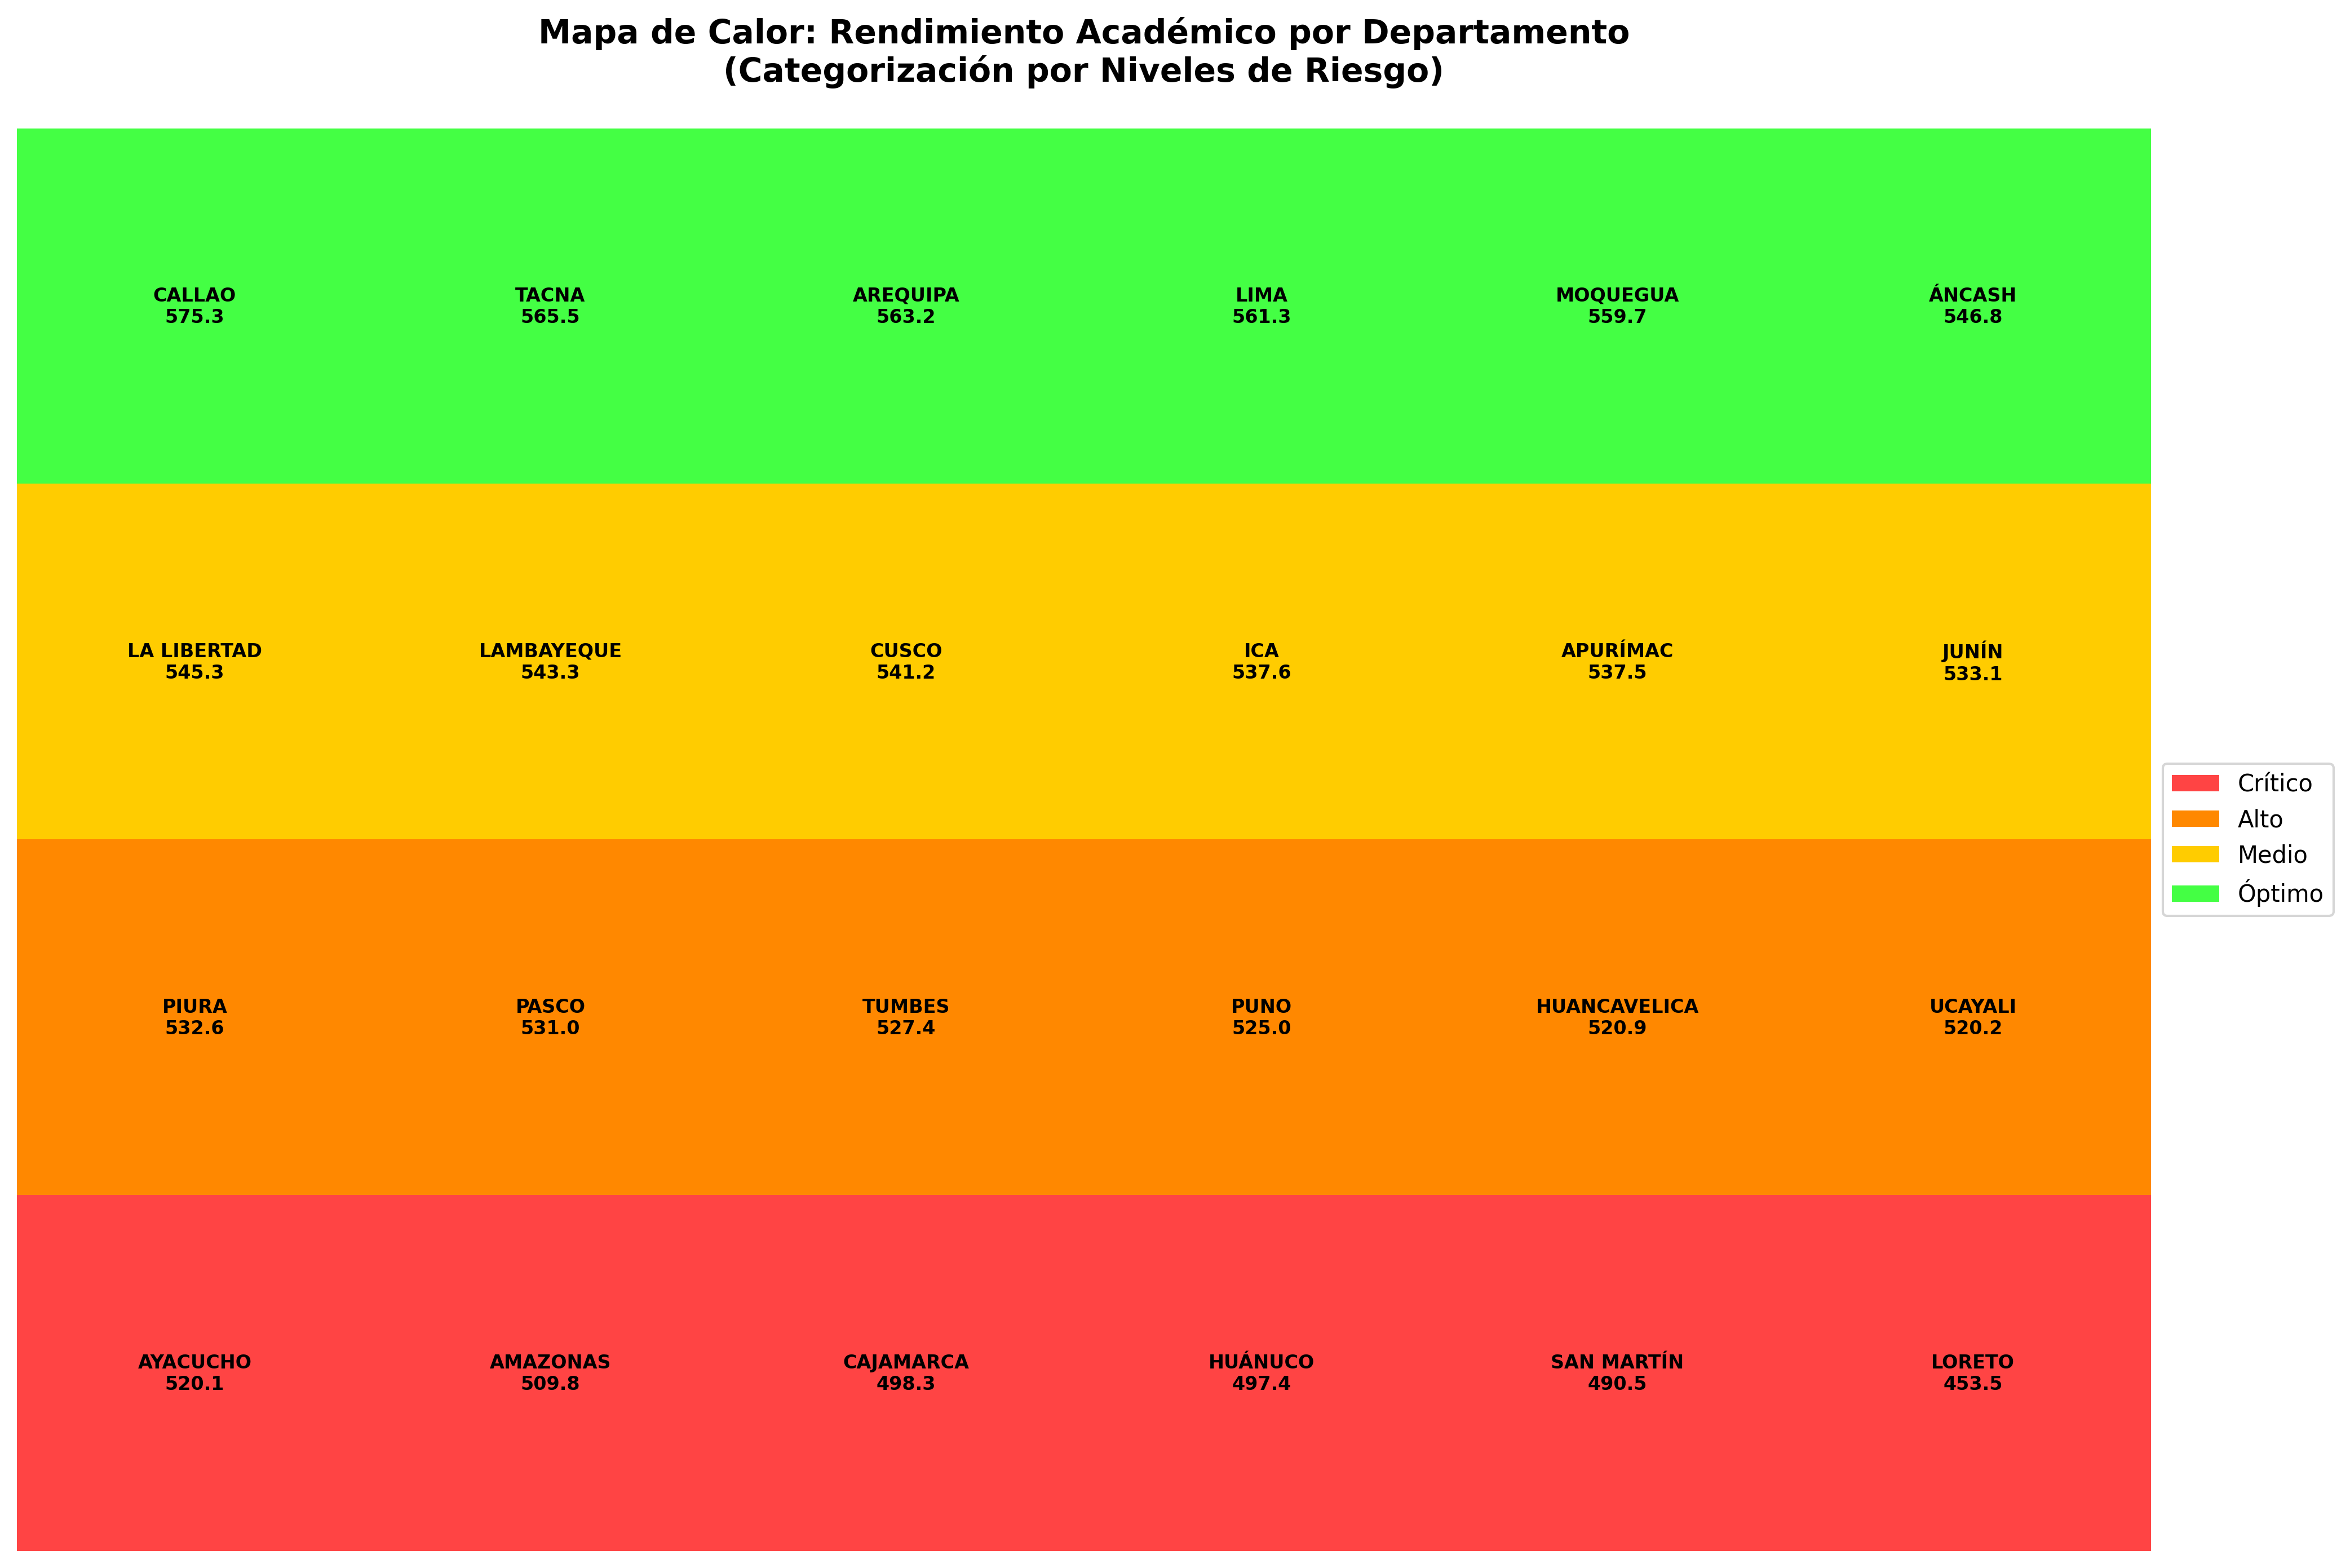
\includegraphics[width=0.45\textwidth]{heatmap_rendimiento_academico.png}}
\caption{Heat map: academic performance categorization by educational risk levels}
\label{fig:heatmap_riesgo}
\end{figure}
Territorial analysis reveals marked geographical stratification of academic performance. Optimal level departments include Callao (575.29), Tacna (565.47), Arequipa (563.16), Lima (561.29), and Moquegua (559.73), corresponding mainly to urban coastal regions with greater economic development and consolidated educational infrastructure. In contrast, departments in critical situation comprise Loreto (453.50), San Martín (490.45), Huánuco (497.41), Cajamarca (498.27), and Amazonas (509.82). These Amazonian and Andean regions face severe structural challenges, including geographical isolation, scarcity of specialized teachers, and limitations in pedagogical resources. The territorial gap between extremes reaches 121.79 points between Callao and Loreto, equivalent to approximately 1.7 years of schooling according to international standards. This disparity evidences profound territorial inequities that reflect structural socioeconomic and geographical inequalities of the Peruvian educational system. The geographical pattern identifies three clearly differentiated corridors: the coastal corridor with optimal performance, characterized by greater urbanization and economic development; the central Andean region with medium performance, where urban and rural factors combine; and the Amazonian region with critical performance, where multiple educational vulnerability factors converge including population dispersion, access limitations, and insufficient resources.

\subsection{Educational Management Analysis}
Results by management type reveal substantial differences between state and non-state institutions. In reading, non-state institutions surpass state ones by 47.19 points (577.54 vs 530.35), while in mathematics the difference reaches 36.64 points (555.93 vs 519.29). This gap reflects disparities in resources, infrastructure, and teacher quality between both sectors. Analysis by mother tongue evidences significant disadvantages for students of indigenous languages. Spanish speakers obtain the best averages (542.60 in reading, 528.74 in mathematics), while students of other indigenous languages present the lowest scores (453.55 in reading, 415.05 in mathematics). This difference of approximately 90 points in reading and 110 in mathematics underscores the challenges of educational inclusion for indigenous populations. These territorial and sociodemographic findings evidence the urgent need to implement territorially differentiated educational policies that prioritize reducing structural gaps, especially in Amazonian regions and indigenous language communities where the greatest inequities of the national educational system are concentrated.

\section{Discussion}

Results provide empirical evidence on methodological equivalence between PSO and Optuna in educational contexts. The observed statistical equivalence (p-values > 0.05) contrasts with literature suggesting superiority of Bayesian methods \cite{bergstra2013making, akiba2019optuna}, attributable to the characteristics of the analyzed two-dimensional search space that allows effective convergence of both algorithms \cite{liu2020improved}. The moderate predictive performance (R² = 0.203 reading, 0.154 mathematics) is consistent with previous studies using sociodemographic variables \cite{romero2020educational, dutt2017systematic}, reflecting the multifactorial nature of academic performance where uncaptured cognitive and pedagogical factors exert determining influence. Territorial analysis reveals systemic inequalities evidenced in the 121.79-point gap between Callao and Loreto, exceeding regional differences reported by UNESCO \cite{unesco2021education} for Latin America. This geographical configuration corroborates unequal development patterns documented \cite{webb2013conexion}, although the magnitude exceeds differences expected by economic factors alone. Segmentation by educational management, where non-state institutions surpass state ones by 47.19 points, confirms privatization effects documented internationally \cite{kremer2013role}. Findings on mother tongue, with 90-point differences between Spanish and indigenous languages, exceed gaps reported in multicultural contexts \cite{garcia2017multilingual}, evidencing limitations in intercultural bilingual education and methodological biases in monolingual evaluations \cite{unesco2016ethnic}. Limitations include absence of educational process variables identified by Peña-Ayala \cite{pena2014educational} and cross-sectional design restrictions noted by Williamson \cite{williamson2020datafication}. The study demonstrates that algorithmic selection can be based on practical considerations rather than theoretical superiority, while the developed territorial approach provides replicable instruments for identifying geographical inequalities and prioritizing interventions in heterogeneous educational systems \cite{gonzalez2023edmcolombia}.

\section{Conclusions}

This research evaluated the comparative effectiveness between Particle Swarm Optimization (PSO) and Bayesian optimization (Optuna) for predicting academic performance of 7839 Peruvian sixth-grade students, using data from the 2022 MINEDU Sample Evaluation. Results demonstrate statistical equivalence between both methods. In reading, PSO achieved MSE of 4872 ± 108 and R² of 0.203 with 116 trees, while Optuna achieved MSE of 4872 ± 106 and R² of 0.203 with 92 trees. In mathematics, PSO recorded MSE of 6650 ± 261 and R² of 0.154 with 180 trees, compared to Optuna which obtained equivalent results using 156 trees. T-tests confirmed absence of significant differences (p-values of 0.940 and 0.821 respectively). Optuna demonstrated greater computational efficiency consistently requiring fewer trees to achieve equivalent performance, positioning itself as the preferable option when resource efficiency is required. PSO constitutes a viable alternative in contexts with specialized framework limitations. The moderate predictive power (20% in reading, 15% in mathematics) reflects the multifactorial nature of academic performance, where pedagogical and family factors not included exert determining influence. Territorial analysis revealed critical inequalities with gaps exceeding 120 points between departments. Coastal regions like Callao (575.29), Tacna (565.47), and Lima (561.29) significantly surpassed Amazonian departments like Loreto (453.50), San Martín (490.45), and Huánuco (497.41). Risk level categorization identified six departments in each level (optimal, medium, high, critical), providing an operational framework for intervention prioritization. The study confirms the determining influence of socioeconomic level, with differences exceeding 80 points between extreme strata, and disparities by educational management where non-state institutions surpass state ones by 47.19 points in reading. Contributions include empirical evidence on metaheuristic algorithm applicability in Latin American educational contexts, demonstrating that PSO can effectively compete with sophisticated Bayesian methods. This finding is especially relevant for institutions with limited resources, as PSO offers accessible implementation without sacrificing predictive effectiveness. Results underscore the need for territorially differentiated educational policies that prioritize gap closure in Amazonian and Andean regions. Validated techniques can be incorporated into early warning systems for national academic performance monitoring, contributing to evidence-based decisions in the Peruvian educational sector. In summary, both PSO and Optuna represent valid tools for educational predictive model optimization, with selection depending on technical capabilities and efficiency requirements. The demonstrated equivalence allows institutions to adopt the approach most suitable to their specific resources, promoting effective implementation of artificial intelligence tools in improving educational quality of the Peruvian system.

\begin{thebibliography}{99}
\bibitem{akiba2019optuna} T. Akiba, S. Sano, T. Yanase, T. Ohta, and M. Koyama, "Optuna: A next-generation hyperparameter optimization framework," \textit{Proceedings of the 25th ACM SIGKDD international conference on knowledge discovery \& data mining}, pp. 2623-2631, 2019.

\bibitem{baker2014educational} R. Baker and P. S. Inventado, "Educational data mining and learning analytics," in \textit{Learning analytics}, Springer, 2014, pp. 61-75.

\bibitem{bergstra2013making} J. Bergstra, D. Yamins, and D. Cox, "Making a science of model search: Hyperparameter optimization in hundreds of dimensions for vision architectures," \textit{International conference on machine learning}, pp. 115-123, 2013.

\bibitem{dietterich1998approximate} T. G. Dietterich, "Approximate statistical tests for comparing supervised classification learning algorithms," \textit{Neural computation}, vol. 10, no. 7, pp. 1895-1923, 1998.

\bibitem{dutt2017systematic} A. Dutt, M. A. Ismail, and T. Herawan, "A systematic review on educational data mining," \textit{IEEE access}, vol. 5, pp. 15991-16005, 2017.

\bibitem{feurer2019hyperparameter} M. Feurer and F. Hutter, "Hyperparameter optimization," in \textit{Automated machine learning}, Springer, 2019, pp. 3-33.

\bibitem{garcia2017multilingual} O. García and L. Wei, "Translanguaging and education," in \textit{Encyclopedia of language and education}, Springer, 2017, pp. 1-14.

\bibitem{gonzalez2023edmcolombia} M. González, P. Rodríguez, and L. Martínez, "Educational data mining in Colombian schools: A particle swarm optimization approach," \textit{Journal of Educational Technology Systems}, vol. 45, no. 2, pp. 123-145, 2023.

\bibitem{kennedy1995particle} J. Kennedy and R. Eberhart, "Particle swarm optimization," \textit{Proceedings of ICNN'95-international conference on neural networks}, vol. 4, pp. 1942-1948, 1995.

\bibitem{kohavi1995study} R. Kohavi, "A study of cross-validation and bootstrap for accuracy estimation and model selection," \textit{International joint Conference on artificial intelligence}, vol. 14, no. 2, pp. 1137-1145, 1995.

\bibitem{kremer2013role} M. Kremer, C. Brannen, and R. Glennerster, "The challenge of education and learning in the developing world," \textit{Science}, vol. 340, no. 6130, pp. 297-300, 2013.

\bibitem{liu2020improved} W. Liu, Z. Wang, X. Liu, N. Zeng, Y. Liu, and F. E. Alsaadi, "A survey of deep neural network architectures and their applications," \textit{Neurocomputing}, vol. 394, pp. 19-28, 2020.

\bibitem{minedu2022em} MINEDU, "Sample Evaluation 2022: Results of the national learning achievement evaluation," \textit{Ministry of Education of Peru}, 2022.

\bibitem{pena2014educational} A. Peña-Ayala, "Educational data mining: A survey and a data mining-based analysis of recent works," \textit{Expert systems with applications}, vol. 41, no. 4, pp. 1432-1462, 2014.

\bibitem{romero2020educational} C. Romero and S. Ventura, "Educational data mining and learning analytics: An updated survey," \textit{Wiley Interdisciplinary Reviews: Data Mining and Knowledge Discovery}, vol. 10, no. 3, p. e1355, 2020.

\bibitem{sultana2021pso} J. Sultana, M. N. Islam, and M. U. Ahmed, "Particle swarm optimization based machine learning approach for student performance prediction," \textit{2021 International Conference on Information Technology}, pp. 1-6, 2021.

\bibitem{unesco2016ethnic} UNESCO, "Ethnic and linguistic minorities in Latin America: Educational challenges and opportunities," \textit{UNESCO Regional Office for Education in Latin America and the Caribbean}, 2016.

\bibitem{unesco2021education} UNESCO, "Education in Latin America and the Caribbean: Regional monitoring report SDG 4," \textit{UNESCO Institute for Statistics}, 2021.

\bibitem{webb2013conexion} R. Webb, "Connection and rural takeoff," \textit{Instituto del Perú, Universidad San Martín de Porres}, 2013.

\bibitem{williamson2020datafication} B. Williamson, "The datafication of education: Algorithmic governance and the digital future of public education," \textit{Policy Press}, 2020.

\bibitem{yang2022optunaed} H. Yang, S. Kim, and J. Park, "Bayesian optimization for educational data mining: An Optuna-based approach," \textit{Educational Technology Research and Development}, vol. 70, no. 3, pp. 789-806, 2022.

\bibitem{zhang2021learning} F. Zhang, J. Li, and X. Wang, "Learning analytics in online learning environments: A systematic review," \textit{Computers \& Education}, vol. 158, p. 104024, 2021.
\end{thebibliography}

\end{document}